\documentclass[xcolor=dvipsnames]{beamer} 
\usepackage{natbib}                 % fancy bibliography.
\usepackage{url}                    % allow printing of urls.
\usepackage{dsfont}
\usepackage{amsmath}
\usepackage{wrapfig}
\usepackage{epstopdf}
\usepackage{listings}

\usepackage{color}

\usepackage{caption}
\setbeamertemplate{footline}[frame number]
\captionsetup{font=scriptsize,labelfont=bf}


\title{\textbf{An introduction to Python}}

\date{}


\definecolor{dkgreen}{rgb}{0,0.6,0}
\definecolor{gray}{rgb}{0.5,0.5,0.5}
\definecolor{mauve}{rgb}{0.58,0,0.82}

\lstset{frame=tb,
  language=Python,
  aboveskip=3mm,
  belowskip=3mm,
  showstringspaces=false,
  columns=flexible,
  basicstyle={\small},
  numbers=none,
  numberstyle=\tiny\color{gray},
  keywordstyle=\color{blue},
  commentstyle=\color{dkgreen},
  stringstyle=\color{mauve},
  breaklines=true,
  breakatwhitespace=true
  tabsize=3
}

\begin{document}
\lstset{language=Python}

\begin{frame}[t]
  \maketitle
  \vskip -9em
\end{frame}

\AtBeginSection[] % Do nothing for \section*
{ 
  \frame<beamer>
    {
          \frametitle{Contents}
	        \tableofcontents[current]
	}
}



\section{Why Python?}

\begin{frame}
\frametitle{Our needs}

\begin{itemize}
\item Get data (simulation, experiment control)
\item Manipulate and process data.
\item Visualize results... to understand what we are doing!
\end{itemize}

\end{frame}


\begin{frame}
\frametitle{What is programming?}

\begin{figure}
\begin{center}
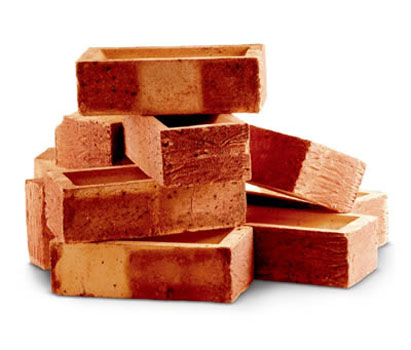
\includegraphics{images/bricks.jpg}
\end{center}
\end{figure}
\end{frame}


\begin{frame}
\frametitle{Why Python?}
\begin{itemize}
\item Readable and well structured language
\item Quick development and execution time
\item Rich collections of existing bricks
\end{itemize}
\end{frame}

\section{The basics}

\begin{frame}
\begin{block}{Value or object}
\frametitle{Values and Data Types}
A \textbf{value} (or an \textbf{object}) is one of the fundamental thing that
a program manipulates. Objects are classified into different \textbf{types} or
\textbf{class}.
\end{block}

\vspace{1em}
\lstinputlisting[language=Python]{src/values.py}
\end{frame}

\begin{frame}
\frametitle{Data Types}

\begin{tabular}{l | l}
boolean & \texttt{True}, \texttt{False} \\
string & \texttt{'Hello world'}, \texttt{"I'm a computer scientist"} \\
integer & \texttt{5} \\
float & \texttt{1.} \\ 
complex & \texttt{1 + 1j}
\end{tabular}

\vspace{1em}
\begin{alertblock}{Question}
\begin{itemize}
\item What is the type of the following values: "3", '5' ?
\end{itemize}
\end{alertblock}
\end{frame}

\begin{frame}
\frametitle{Using Python as a calculator}

The \textbf{interpreter} can be used as a simple calculator.

\vspace{1em}
\lstinputlisting[language=Python]{src/calculator.py}

\vspace{1em}
\begin{alertblock}{Question}
\begin{itemize}
\item Do you understand all the outputs?
\item What do you think the pound (\texttt{\#}) sign means?
\end{itemize}
\end{alertblock}
\end{frame}


\begin{frame}
\frametitle{Using Python to compare}

Several operators (\texttt{>}, \texttt{==}, \texttt{!=}, \texttt{<=}) can be
used to compared values of same or different types.

\vspace{1em}
\lstinputlisting[language=Python]{src/comparison.py}
\end{frame}

\begin{frame}
\frametitle{Variables and assignments}
\begin{block}{Variables}

A \textbf{variable} is a name that refers to a value.
A value is \textbf{assigned} to a variable.
\end{block}
\vspace{1em}
\lstinputlisting[language=Python]{src/variables.py}

\vspace{1em}
\begin{alertblock}{Question}
\begin{itemize}
\item What are the types of \texttt{a} and \texttt{b}?
\item What is the type of \texttt{c}?
\end{itemize}
\end{alertblock}
\end{frame}

\begin{frame}
\frametitle{Variables and assigments}
\begin{itemize}
\item A variable is just a name.
\item You must assign a value to a variable before using it.
\end{itemize}
\lstinputlisting{src/variables_1.py}
\end{frame}

\begin{frame}
\frametitle{A few Python built-in functions}

\begin{block}{Function}
A \textbf{function} is a block of code that takes in input no, one or many \textbf{arguments}
and returns something (often a value).
\end{block}

\begin{minipage}[tl]{0.45\textwidth}
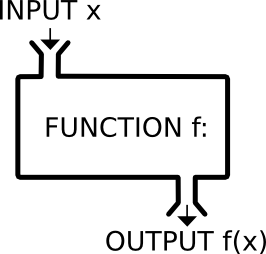
\includegraphics[width=60px]{images/Function_machine2.png}
\end{minipage}

\begin{minipage}[tr]{0.45\textwidth}
\lstinputlisting{src/builtins.py}
\end{minipage}
\end{frame}

\begin{frame}
\frametitle{A few Python built-ins}
\scriptsize
\begin{tabular}{lllll}
\texttt{abs()} & \texttt{divmod()} & \texttt{input()} & \texttt{open()} & \texttt{staticmethod()} \\
\texttt{all()} & \texttt{enumerate()} & \texttt{int()} & \texttt{ord()} & \texttt{str()} \\
\texttt{any()} & \texttt{eval()} & \texttt{isinstance()} & \texttt{pow()} & \texttt{sum()} \\
\texttt{basestring()}  &   \texttt{execfile()}  &   \texttt{issubclass()}  &   \texttt{print()}  &   \texttt{super()} \\
\texttt{bin()}  &   \texttt{file()}  &   \texttt{iter()}  &   \texttt{property()}  &   \texttt{tuple()} \\
\texttt{bool()}  &   \texttt{filter()}  &   \texttt{len()}  &   \texttt{range()}  &   \texttt{type()} \\
\texttt{bytearray()}  &   \texttt{float()}  &   \texttt{list()}  &   \texttt{raw\_input()}  &   \texttt{unichr()} \\
\texttt{callable()}  &   \texttt{format()}  &   \texttt{locals()}  &   \texttt{reduce()}  &   \texttt{unicode()} \\
\texttt{chr()}  &   \texttt{frozenset()}  &   \texttt{long()}  &   \texttt{reload()}  &   \texttt{vars()} \\
\texttt{classmethod()}  &   \texttt{getattr()}  &   \texttt{map()}  &   \texttt{repr()}  &   \texttt{xrange()} \\
\texttt{cmp()}  &   \texttt{globals()}  &   \texttt{max()}  &   \texttt{reversed()}  &   \texttt{zip()} \\
\texttt{compile()}  &   \texttt{hasattr()}  &   \texttt{memoryview()}  &   \texttt{round()}  & \texttt{\_\_import\_\_()} \\
\texttt{complex()}  &   \texttt{hash()}  &   \texttt{min()}  &   \texttt{set()}  &   \texttt{apply()} \\
\texttt{delattr()}  &   \texttt{help()}  &   \texttt{next()}  &   \texttt{setattr()}  &   \texttt{buffer()} \\
\texttt{dict()}  &   \texttt{hex()}  &   \texttt{object()}  &   \texttt{slice()}  &   \texttt{coerce()} \\
\texttt{dir()}  &   \texttt{id()}  &   \texttt{oct()}  &   \texttt{sorted()}  &   \texttt{intern()} \\
\end{tabular}
\end{frame}

\begin{frame}
\frametitle{A few Python built-ins}
\scriptsize
\begin{tabular}{lllll}
\texttt{abs()} & \texttt{divmod()} & \texttt{input()} & \texttt{open()} & \texttt{staticmethod()} \\
\texttt{all()} & \texttt{enumerate()} & {\color{blue} \texttt{int()}} & \texttt{ord()} & {\color{blue} \texttt{str()}} \\
\texttt{any()} & \texttt{eval()} & \texttt{isinstance()} & \texttt{pow()} & \texttt{sum()} \\
\texttt{basestring()}  &   \texttt{execfile()}  &   \texttt{issubclass()}  &   \texttt{print()}  &   \texttt{super()} \\
\texttt{bin()}  &   \texttt{file()}  &   \texttt{iter()}  &   \texttt{property()}  &   \texttt{tuple()} \\
{\color{blue} \texttt{bool()}} &   \texttt{filter()}  &   \texttt{len()}  &   \texttt{range()}  &   \texttt{type()} \\
\texttt{bytearray()}  & {\color{blue} \texttt{float()}} &   \texttt{list()}  &   \texttt{raw\_input()}  &   \texttt{unichr()} \\
\texttt{callable()}  &   \texttt{format()}  &   \texttt{locals()}  &   \texttt{reduce()}  &   \texttt{unicode()} \\
\texttt{chr()}  &   \texttt{frozenset()}  &   \texttt{long()}  &   \texttt{reload()}  &   \texttt{vars()} \\
\texttt{classmethod()}  &   \texttt{getattr()}  &   \texttt{map()}  &   \texttt{repr()}  &   \texttt{xrange()} \\
\texttt{cmp()}  &   \texttt{globals()}  &   \texttt{max()}  &   \texttt{reversed()}  &   \texttt{zip()} \\
\texttt{compile()}  &   \texttt{hasattr()}  &   \texttt{memoryview()}  &   \texttt{round()}  & \texttt{\_\_import\_\_()} \\
{\color{blue} \texttt{complex()}} &   \texttt{hash()}  &   \texttt{min()}  &   \texttt{set()}  &   \texttt{apply()} \\
\texttt{delattr()}  &   \texttt{help()}  &   \texttt{next()}  &   \texttt{setattr()}  &   \texttt{buffer()} \\
\texttt{dict()}  &   \texttt{hex()}  &   \texttt{object()}  &   \texttt{slice()}  &   \texttt{coerce()} \\
\texttt{dir()}  &   \texttt{id()}  &   \texttt{oct()}  &   \texttt{sorted()}  &   \texttt{intern()} \\
\end{tabular}
\end{frame}

\begin{frame}
\frametitle{A few Python built-ins}
\scriptsize
\begin{tabular}{lllll}
\texttt{abs()} & \texttt{divmod()} & \texttt{input()} & \texttt{open()} & \texttt{staticmethod()} \\
\texttt{all()} & \texttt{enumerate()} & {\color{blue} \texttt{int()}} & \texttt{ord()} & {\color{blue} \texttt{str()}} \\
\texttt{any()} & \texttt{eval()} & \texttt{isinstance()} & \texttt{pow()} & \texttt{sum()} \\
\texttt{basestring()}  &   \texttt{execfile()}  &   \texttt{issubclass()}  &   \texttt{print()}  &   \texttt{super()} \\
\texttt{bin()}  &   \texttt{file()}  &   \texttt{iter()}  &   \texttt{property()}  &   \texttt{tuple()} \\
{\color{blue} \texttt{bool()}} &   \texttt{filter()}  &   \texttt{len()}  &   \texttt{range()}  &   \texttt{type()} \\
\texttt{bytearray()}  & {\color{blue} \texttt{float()}} &   \texttt{list()}  &   \texttt{raw\_input()}  &   \texttt{unichr()} \\
\texttt{callable()}  &   \texttt{format()}  &   \texttt{locals()}  &   \texttt{reduce()}  &   \texttt{unicode()} \\
\texttt{chr()}  &   \texttt{frozenset()}  & {\color{blue} \texttt{long()}} &   \texttt{reload()}  &   \texttt{vars()} \\
\texttt{classmethod()}  &   \texttt{getattr()}  &   \texttt{map()}  &   \texttt{repr()}  &   \texttt{xrange()} \\
\texttt{cmp()}  &   \texttt{globals()}  &   \texttt{max()}  &   \texttt{reversed()}  &   \texttt{zip()} \\
\texttt{compile()}  &   \texttt{hasattr()}  &   \texttt{memoryview()}  &   \texttt{round()}  & \texttt{\_\_import\_\_()} \\
{\color{blue} \texttt{complex()}} &   \texttt{hash()}  &   \texttt{min()}  &   \texttt{set()}  &   \texttt{apply()} \\
\texttt{delattr()}  &   \texttt{help()}  &   \texttt{next()}  &   \texttt{setattr()}  &   \texttt{buffer()} \\
\texttt{dict()}  &   \texttt{hex()}  &   \texttt{object()}  &   \texttt{slice()}  &   \texttt{coerce()} \\
\texttt{dir()}  &   \texttt{id()}  &   \texttt{oct()}  &   \texttt{sorted()}  &   \texttt{intern()} \\
\end{tabular}
\end{frame}

\begin{frame}
\frametitle{A few Python built-ins}
\scriptsize
\begin{tabular}{lllll}
\texttt{abs()} & \texttt{divmod()} & \texttt{input()} & \texttt{open()} & \texttt{staticmethod()} \\
\texttt{all()} & \texttt{enumerate()} & {\color{blue} \texttt{int()}} & \texttt{ord()} & {\color{blue} \texttt{str()}} \\
\texttt{any()} & \texttt{eval()} & \texttt{isinstance()} & \texttt{pow()} & \texttt{sum()} \\
\texttt{basestring()}  &   \texttt{execfile()}  &   \texttt{issubclass()}  &   \texttt{print()}  &   \texttt{super()} \\
\texttt{bin()}  &   \texttt{file()}  &   \texttt{iter()}  &   \texttt{property()}  &   \texttt{tuple()} \\
\texttt{bool()}  &   \texttt{filter()}  &   \texttt{len()}  &   \texttt{range()}  &   \texttt{type()} \\
\texttt{bytearray()}  & {\color{blue} \texttt{float()}} &   \texttt{list()}  &   \texttt{raw\_input()}  &   \texttt{unichr()} \\
\texttt{callable()}  &   \texttt{format()}  &   \texttt{locals()}  &   \texttt{reduce()}  &   \texttt{unicode()} \\
\texttt{chr()}  &   \texttt{frozenset()}  & {\color{blue} \texttt{long()}} &   \texttt{reload()}  &   \texttt{vars()} \\
\texttt{classmethod()}  &   \texttt{getattr()}  &   \texttt{map()}  &   \texttt{repr()}  &   \texttt{xrange()} \\
\texttt{cmp()}  &   \texttt{globals()}  & {\color{red} \texttt{max()}} &   \texttt{reversed()}  &   \texttt{zip()} \\
\texttt{compile()}  &   \texttt{hasattr()}  &   \texttt{memoryview()}  &   \texttt{round()}  & \texttt{\_\_import\_\_()} \\
{\color{blue} \texttt{complex()}} &   \texttt{hash()}  & {\color{red} \texttt{min()}} &   \texttt{set()}  &   \texttt{apply()} \\
\texttt{delattr()}  &   \texttt{help()}  &   \texttt{next()}  &   \texttt{setattr()}  &   \texttt{buffer()} \\
\texttt{dict()}  &   \texttt{hex()}  &   \texttt{object()}  &   \texttt{slice()}  &   \texttt{coerce()} \\
\texttt{dir()}  &   \texttt{id()}  &   \texttt{oct()}  &   \texttt{sorted()}  &   \texttt{intern()} \\
\end{tabular}
\end{frame}

\begin{frame}
\frametitle{A few Python built-ins}
\scriptsize
\begin{tabular}{lllll}
\texttt{abs()} & \texttt{divmod()} & \texttt{input()} & \texttt{open()} & \texttt{staticmethod()} \\
\texttt{all()} & \texttt{enumerate()} & \texttt{int()} & \texttt{ord()} & \texttt{str()} \\
\texttt{any()} & \texttt{eval()} & \texttt{isinstance()} & \texttt{pow()} & \texttt{sum()} \\
\texttt{basestring()}  &   \texttt{execfile()}  &   \texttt{issubclass()}  &   \texttt{print()}  &   \texttt{super()} \\
\texttt{bin()}  &   \texttt{file()}  &   \texttt{iter()}  &   \texttt{property()}  &   \texttt{tuple()} \\
\texttt{bool()}  &   \texttt{filter()}  &   \texttt{len()}  &   \texttt{range()}  &   \texttt{type()} \\
\texttt{bytearray()}  &   \texttt{float()}  &   \texttt{list()}  &   \texttt{raw\_input()}  &   \texttt{unichr()} \\
\texttt{callable()}  &   \texttt{format()}  &   \texttt{locals()}  &   \texttt{reduce()}  &   \texttt{unicode()} \\
\texttt{chr()}  &   \texttt{frozenset()}  &   \texttt{long()}  &   \texttt{reload()}  &   \texttt{vars()} \\
\texttt{classmethod()}  &   \texttt{getattr()}  &   \texttt{map()}  &   \texttt{repr()}  &   \texttt{xrange()} \\
\texttt{cmp()}  &   \texttt{globals()}  &   \texttt{max()}  &   \texttt{reversed()}  &   \texttt{zip()} \\
\texttt{compile()}  &   \texttt{hasattr()}  &   \texttt{memoryview()}  &   \texttt{round()}  & \texttt{\_\_import\_\_()} \\
\texttt{complex()}  &   \texttt{hash()}  &   \texttt{min()}  &   \texttt{set()}  &   \texttt{apply()} \\
\texttt{delattr()}  & {\color{green} \texttt{help()}} &   \texttt{next()}  &   \texttt{setattr()}  &   \texttt{buffer()} \\
\texttt{dict()}  &   \texttt{hex()}  &   \texttt{object()}  &   \texttt{slice()}  &   \texttt{coerce()} \\
{\color{green} \texttt{dir()}} &   \texttt{id()}  &   \texttt{oct()}  &   \texttt{sorted()}  &   \texttt{intern()} \\
\end{tabular}
\end{frame}

\begin{frame}
\frametitle{What about \texttt{print} ?}
\end{frame}

\begin{frame}
\frametitle{Exercises}
\begin{itemize}
\item \textbf{Q1} What is printed when the following statements are executed?
\lstinputlisting{src/Q01.py}
\item \textbf{Q2} How would you swap the values of two variables \texttt{a}
and \texttt{b}?
\item \textbf{Q3} Use the function \texttt{help} on the function \texttt{file}
to find out what it does.
\item \textbf{Q4} Is the string \textbf{"attaccgtga"} of length a multiple of
3 ?
\item \textbf{Q5} run \texttt{dir("at")}. Can you guess what the function
\texttt{dir} does?
\end{itemize}
\end{frame}

\begin{frame}
\frametitle{Manipulation on strings}

Let \texttt{s} be a string: \texttt{s = "Hello world! "}.

\begin{table}
\scriptsize
\begin{tabular}{lcl}
Method & Returns & Description \\
\hline
\texttt{s.count("o")} & \texttt{2} & Return the number of occurence of \\
		      &		   & the substring. \\
\texttt{s.split(" ")} & {\tiny \texttt{['Hello', 'world!', '']}} & Split on the substring \\
\texttt{s.startswith("H")} & \texttt{True} & Return whether s starts with the
substring \\
\texttt{s.endswith("H")} & \texttt{False} & Return whether s ends with the
substring \\
\texttt{s.strip()} & \texttt{"Hello world!} & Remove trailing whitespace \\
\texttt{s.lower()} & \texttt{"hello world! "} & Return lowercase version of
the string \\
\end{tabular}
\end{table}

\vspace{1em}
\lstinputlisting{src/string_manipulation.py}
\end{frame}

\begin{frame}
\frametitle{Manipulation on strings}
Strings can be
\begin{itemize}
\item \textbf{indexed}: indexes starts at 0.
\lstinputlisting{src/string_manipulation_1.py}
\item \textbf{sliced}: selects a subset of the string.
\lstinputlisting{src/string_manipulation_2.py}
\end{itemize}
\end{frame}

\begin{frame}
\frametitle{Saving and running Python scripts}
\begin{block}{Script}
A \textbf{script}:
\begin{itemize}
\item is a file containing python code, ending by \texttt{.py}
\item can be run in a shell using \texttt{python filename.py}
\end{itemize}
\end{block}

\begin{alertblock}{Text editor}
It is important to have a good text editor. We will use \textbf{spyder}.
\begin{center}

\includegraphics[width=50px]{images/spyder.jpg}
\end{center}
\end{alertblock}
\end{frame}

\section{Containers and control flow}
\begin{frame}
\frametitle{So far...}
\begin{block}{We have seen...}
\begin{itemize}
\item Basic types (\texttt{int}, \texttt{float}, \texttt{strings...})
\item How to manipulate strings and numerical types
\item How to write and run a script
\end{itemize}
\end{block}
\end{frame}

\begin{frame}
\frametitle{And now}
\begin{columns}

% FIXME
\begin{column}{0.5\textwidth}
\begin{block}{Repetition}
\end{block}
\end{column}

\begin{column}{0.5\textwidth}
\begin{block}{Selection}
\end{block}
\end{column}
\end{columns}
\end{frame}

\begin{frame}
\frametitle{Repetition}
\lstinputlisting{src/while.py}
\end{frame}

\begin{frame}
\frametitle{Repetition}
\lstinputlisting{src/while_1.py}
\end{frame}

\begin{frame}
\frametitle{Repetition}
\lstinputlisting{src/while_2.py}
\end{frame}

\begin{frame}
\frametitle{Selection}
\lstinputlisting{src/if_elif_else.py}
\end{frame}

\begin{frame}
\frametitle{Exercises}
\begin{itemize}
\item \textbf{Q1} Write a small script that prints whether the product of two
variables \texttt{a} and \texttt{b} is negative, null or positive.
\item \textbf{Q2} Rewrite this without computing the
product of those two variables.
\item \textbf{Q3} Find the 100th element of the Fibonacci suite ($F_0 = 0$,
$F_1 = 1$, $F_{n + 1} = F_n + F_{n - 1}$)
\item \textbf{Q4} 
Write a program that prints the numbers from 1 to 100. But for multiples of
three print "Fizz" instead of the number and for the multiples of five print
"Buzz". For numbers which are multiples of both three and five print
"FizzBuzz".
\end{itemize}
\end{frame}

\begin{frame}
\frametitle{Containers}

\end{frame}

\begin{frame}
\frametitle{Looping}
\end{frame}

\end{document}
